\chapter{Theory}


\section{Machine Learning and Computer Vision}
\subsection{Types of Models}
ml is used for ....
types of models
..
neural networks

\subsection{Computer Vision}
use and so on, how works,
our opencv library
rgb gbr conversion

\section{Mediapipe}
company, availability, types of models, what they offer, devices options, what we use

\subsection{Input Image Processing}
color, background, extracting lanmarks for mediapipe model no. 2, with vs without Mediapipe

\subsection{MediaPipe and hand landmark detection}

MediaPipe is a framework used to create machine learning pipelines for time-series data like video and audio. Google initially developed it to process real-time video and audio analysis on YouTube. In 2019, the public release allowed researchers and developers to incorporate MediaPipe into their projects. Unlike other machine learning frameworks that require high computing power, MediaPipe can run efficiently on devices with low power, such as Android and IoT devices. It consists of the MediaPipe framework and MediaPipe solutions. The MediaPipe framework is developed using C++, Java, and Objective C programming. MediaPipe solutions include 16 pre-trained TensorFlow and TensorFlow Lite models built on top of the MediaPipe framework for specific use cases. This work used the MediaPipe solution to identify 21 3D landmark points on a hand from a single frame of a hand sign image. To achieve this, two dependent models are used simultaneously. First, a Palm Detection Model detects the palms of hands in the images since it is easier to detect rigid objects like palms and fists rather than a complete hand. Cropped palm images from this model are passed onto the next model, which is the Hand Landmark Model. The model accurately detects 21 3D hand landmark points in the detected hand region using regression. It is trained on approximately 30,000 manually annotated real-world images and is very well-trained and robust, allowing it to detect and map hand landmark points accurately, even on partially visible hands in most cases.


\begin{figure}
	\centering
	\includegraphics[width = \textwidth]{images/all_gestures.pdf}
	\caption{Gestures used in the project}
	\label{fig:all_gestures}
\end{figure}





\subsubsection{Data Normalization}
The MediaPipe hand landmarks model provides coordinates for hand landmark points based on the position of pixels containing those points in an image. As a result, the coordinates of two images of the same hand sign with different placements in the frame can have significantly different distances between them. This makes it more challenging to train the model.

 To solve this problem, the wrist's landmark point has been considered with coordinates (0,0), and the coordinates of all other landmark points were adjusted accordingly.
First, the coordinates' values of the wrist's landmark point are subtracted from all coordinates' values. 


 Then, the coordinates were normalized to be between 0 and 1 by dividing them by the largest absolute value of the difference. Finally, the normalized coordinates were collected in the landmarks list. The coordinate normalization procedure is shown in Fig \ref{fig:normalization}.
\begin{figure}
	\centering
	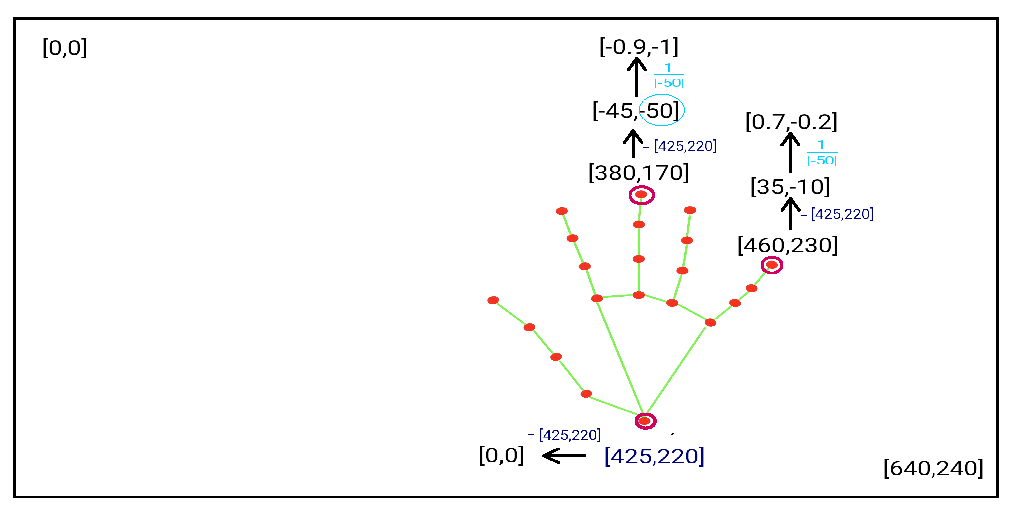
\includegraphics[width = 0.85\textwidth]{images/normalise.pdf}
	\caption{Process of normalization of landmark coordinates}
	\label{fig:normalization}
\end{figure}




\section{Gesture Recognition}

The process of recognizing hand gestures as input, mapping them to a representation, and converting them into a purposeful command for devices is known as gesture recognition. The goal is to identify and process explicit hand gestures for output. 
Dynamic gestures refer to a sequence of poses that change over time, while static gestures remain constant. Static hand gestures can be classified based on their temporal relationship and recognized by analyzing features such as spatial position, orientation, contour, and texture. We will focus on recognizing static gestures using a vision-based method.


tu nejake obrazky na classification

\section{Drone Control}



